% !TEX program = xelatex
\DocumentMetadata{} % required for transparent package
\documentclass[12pt,aspectratio=169]{beamer}

\makeatletter
\def\@makefnmark{}
\makeatletter

\setbeamersize{text margin left=5mm,text margin right=5mm} 

\newcommand\focus[1]{%
	{\alert{\textbf{#1}}}
}

\usepackage{amsthm,amsmath,amssymb,braket,fontspec,unicode-math,fontenc,transparent}
\usepackage[absolute,overlay]{textpos}

\usetheme{moloch}
\setmainfont{SF Pro Display}
\setsansfont{SF Pro Display}
\setmathfont{Fira Math}
\setmathfont{latinmodern-math.otf}[range={frak,\bigcap,\bigcup}]

\usepackage[backend=bibtex,url=false,doi=false,style=authoryear]{biblatex}
\setbeamertemplate{bibliography item}{}
\bibliography{bib}
\AtBeginBibliography{\scriptsize}

\graphicspath{{./figures/}}

\title{Research Progress Report: 2023 - 2024}

\author{Abhirup Mukherjee}
\institute{
Department of Physical Sciences,\\
IISER Kolkata, Mohanpur}

\begin{document}

\centering

\begin{frame}
\maketitle
\end{frame}

\begin{frame}{Publications and Ongoing projects}
\focus{Currently in progress}
\begin{itemize}
	\item Development of a new auxiliary model-based method for studying systems of interacting electronics.\\[10pt]
	\item Studies of the plateau-to-plateau transition in integer quantum hall systems.
\end{itemize}

\vspace*{\fill}

\focus{Published}
\begin{itemize}
	\item Abhirup Mukherjee et al 2023 New J. Phys. 25 113011
	\item Abhirup Mukherjee et al 2024 J. Phys. A: Math. Theor. 57 275401\\[10pt]
	\item \transparent{0.4}{Anirban Mukherjee et al 2022 Phys. Rev. B 105, 085119}
	\item \transparent{0.4}{Siddhartha Patra et al 2023 J. Phys.: Condens. Matter 35 315601}
\end{itemize}

\end{frame}

\section{Project I: A New Auxiliary Model Approach to Systems of Interacting Electrons}
\subsection{Ongoing project}

\begin{frame}{Broad Objectives}

\begin{itemize}
	\item Designing a \focus{new method} by which to leverage quantum impurity models towards studying lattice models of interacting electrons\\[10pt]
	\item Using such a method to go after the \focus{Mott-Hubbard MIT} on the 2D square lattice\\[10pt]
	\item Capturing the enhanced effects of \focus{\(k-\)space anisotropy} (due to the square lattice) on signatures near the transition\\[10pt]
	\item Studying the (presumably) \focus{non-Fermi liquid behaviour} in the excitations close to and at the transition
\end{itemize}

\end{frame}

\begin{frame}{Momentum-Resolved Renormalisation Group Flows}
\begin{minipage}{0.25\textwidth}
	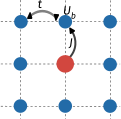
\includegraphics[width=\textwidth]{pWaveEsiam.pdf}
\end{minipage}
\hspace*{\fill}
\begin{minipage}{0.45\textwidth}
	Hamiltonian RG equations of \\
	\focus{embedded e-SIAM}\\
	\(\Delta J^{(j)}_{{\bf k}_1, {\bf k}_2} = -\sum_{{\bf q} \in \text{PS}} \frac{J^{(j)}_{{\bf k}_2,{\bf q}} J^{(j)}_{{\bf q},{\bf k}_1} + 4J^{(j)}_{{\bf q}, {\bf \bar q}} W_{{\bf \bar q}, {\bf k}_2, {\bf k}_1, {\bf q}}}{\omega - \frac{1}{2}|\varepsilon_j| + J^{(j)}_{{\bf q}}/4 + W_{{\bf q}}/2}\)
\end{minipage}
\hspace*{\fill}
\begin{minipage}{0.25\textwidth}
	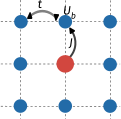
\includegraphics[width=\textwidth]{pWaveEsiam.pdf}
\end{minipage}

\vspace*{\fill}
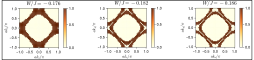
\includegraphics[width=0.9\textwidth]{scattProb.pdf}
	
\end{frame}

\begin{frame}{`Periodising' the Hamiltonian and Eigenstates}
	\begin{minipage}{0.45\textwidth}
		Periodising the Hamiltonian creates a \focus{Hubbard-Heisenberg} model:
	\begin{equation*}\begin{aligned}
		\mathcal{H}_\text{tiled} =& \sum_{{\bf r}}T^\dagger({\bf r} - {\bf r}_d)\mathcal{H}_\text{aux}({\bf r}_d)T({\bf r} - {\bf r}_d)\\
	\end{aligned}\end{equation*}
	\end{minipage}
	\hspace{\fill}
	\begin{minipage}{0.45\textwidth}
		Wavefunctions can be related using a many-body \focus{Bloch's theorem}:
	\[\ket{\Psi_\text{gs}} = \frac{1}{\sqrt N}\sum_{{\bf r}_d} e^{i {\bf k}\cdot{\bf r}_d} \ket{\psi_\text{gs}\left({\bf r}_d\right)}\]

	\end{minipage}

	\vspace*{\fill}
	\(H_\text{tiled} = -\frac{\tilde t}{\sqrt{\mathcal{Z}}}\sum_{\left<{\bf r}_i, {\bf r}_j\right>;\sigma}\left(c^\dagger_{{\bf r}_i,\sigma}c_{{\bf r}_j,\sigma} + \text{h.c.}\right) + \frac{\tilde J}{\mathcal{Z}}\sum_{\left< {\bf r}_i, {\bf r}_j\right>}{\bf S}_{{\bf r}_i}\cdot{\bf S}_{{\bf r}_j} - \frac{\tilde U}{2}\sum_{\bf r}\left(\hat n_{{\bf r} , \uparrow} - \hat n_{{\bf r} , \downarrow}\right)^2\)

	\vspace*{15pt}
	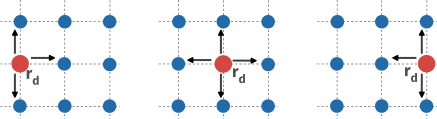
\includegraphics[width=0.8\textwidth]{periodisation.pdf}
	
\end{frame}

\begin{frame}{Periodising the Greens Functions}
	\begin{minipage}{0.4\textwidth}
	Greens function = \\
	sum of 1-particle \focus{\(k-\)space} Greens functions starting from \focus{all sites} in impurity model.
	\end{minipage}
	\hspace{\fill}
	\begin{minipage}{0.54\textwidth}
	\begin{equation*}\begin{aligned}
		\tilde G({\bf r}; \tilde\omega) = \frac{1}{N}\sum_{{\bf k},{\bf r}_x} \left[e^{i \left({\bf k}- {\bf k}_0\right)\cdot\left({\bf r} - {\bf r}_x\right)}G_p\left({\bf r}_x;\omega + \varepsilon_{\bf k}\right) \right. \\
	\left. + e^{-i \left({\bf k}- {\bf k}_0\right)\cdot\left({\bf r} - {\bf r}_x\right)}G_h\left({\bf r}_x;\omega - \varepsilon_{\bf k}\right)\right]
	\end{aligned}\end{equation*}
	\end{minipage}

	\vspace*{\fill}
	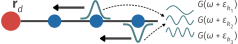
\includegraphics[width=0.8\textwidth]{greensFunc.pdf}

	\vspace*{\fill}
	\begin{minipage}{0.45\textwidth}
	\(\tilde A({\bf K}; \omega )= -\frac{1}{\pi}\text{Im}\left[\tilde G({\bf K}; \tilde\omega)\right]\)\\
	\(\tilde \Sigma({\bf K}; \omega) = \left(\tilde G^{(0)}({\bf K}; \tilde\omega)\right)^{-1} - \left(\tilde G({\bf K}; \tilde\omega)\right)^{-1}\)
	\end{minipage}
	\hspace{\fill}
	\begin{minipage}{0.5\textwidth}
	Subsequently allows periodising spectral \\ 
	functions and self-energies
	\end{minipage}
	
\end{frame}

\begin{frame}{Periodising Correlation Functions and Entanglement Measures}
	\begin{minipage}{0.49\textwidth}
	\(k-\)space spin-spin correlation
	\begin{equation*}\begin{aligned}
	&\tilde{S}_\text{flip}({\bf K}_1, {\bf K}_2) = \\
	&\frac{1}{2}\left[\sqrt{\braket{S^+\left({\bf d}\right)S^-\left({\bf K}_2\right)}\braket{S^-\left({\bf d}\right)S^+\left({\bf K}_1\right)}} + \text{h.c.}\right]
	\end{aligned}\end{equation*}
	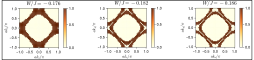
\includegraphics[width=\textwidth]{scattProb.pdf}
	\end{minipage}
	\begin{minipage}{0.49\textwidth}
	\(k-\)space reduced density matrix
	\begin{equation*}\begin{aligned}
		&\overline\rho_{{\bf K},\sigma} = \frac{1}{2}\left[c^\dagger_{{\bf K},\sigma} \rho_\text{gs}({\bf r}_c) c_{{\bf r}_c,\sigma} + c^\dagger_{{\bf r}_c,\sigma} \rho_\text{gs}({\bf r}_c) c_{{\bf K},\sigma}\right] \\
		& + \text{h.c.}
	\end{aligned}\end{equation*}
	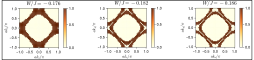
\includegraphics[width=\textwidth]{scattProb.pdf}
	\end{minipage}
	
\end{frame}

\begin{frame}{What Remains}
	\begin{itemize}
		\item Calculating of spectral functions and self-energies
		\item Characterisation of non-Fermi liquid behaviour in the pseudogapped region
	\end{itemize}
\end{frame}

\section{Search for punctured-Chern topology at IQHE transitions}
\subsection{Ongoing project}

\begin{frame}{Broad questions}

\vspace*{\fill}
\begin{minipage}{0.5\textwidth}
\begin{itemize}[<+->]
	\item Obtaining the \alert{IQHE phase diagram} from a model of 2D lattice electrons\\[10pt]
	\item Understanding the \alert{topology} of the ground state precisely at a transition\\[10pt]
	\item Extending this to systems with \alert{disorder} and interactions.
\end{itemize}
\end{minipage}
\hspace*{\fill}
\begin{minipage}{0.4\textwidth}
% 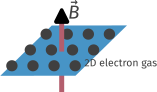
\includegraphics[width=\textwidth]{IQHE.pdf}
\end{minipage}

\vspace*{\fill}
\end{frame}

\begin{frame}{Preliminary results}
Emergence of \alert{Landau levels} in a magnetic field is similar to the formation of \alert{bands} in a periodic potential.

\vspace*{\fill}
% 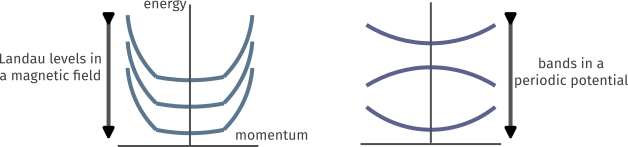
\includegraphics[width=\textwidth]{bands.pdf}

\vspace*{\fill}
We first studied the simpler problem of \alert{particle in a periodic potential}.
\end{frame}

\begin{frame}{Preliminary results}
We first studied the simpler problem of \alert{particle in a periodic potential}.

\vspace*{\fill}
% 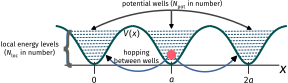
\includegraphics[width=0.8\textwidth]{potential.pdf}

\vspace*{\fill}
	
\begin{itemize}
	\item Can understand the formation of bands under RG
	\item Obtained insights regarding the \alert{effective center of mass} degrees of freedom
	\item Needs to be extended by incorporating a \alert{magnetic field}
\end{itemize}
\end{frame}

\section{Summary}
\subsection{~}

\begin{frame}{Summary}
\alert{Currently in progress}\\
\begin{itemize}
	\item Development of auxiliary model-based method for studying bulk correlated systems.\\[10pt]
	\item Studies of the plateau-to-plateau transition in integer quantum hall systems.
\end{itemize}

\vspace*{\fill}
\hrule

\vspace*{\fill}
\begin{minipage}{0.55\textwidth}
\begin{itemize}
	\item[$\checkmark$] 2022 \alert{Phys. Rev. B} 105, 085119.\\ A Mukherjee, \alert{Abhirup Mukherjee}, \ldots, S. Lal\\[10pt]
	\item[$\checkmark$] 2023 \alert{J. Phys.: Condens. Matter} 35 315601.\\ S Patra, \alert{Abhirup Mukherjee}, \ldots, S. Lal
\end{itemize}
\end{minipage}
\begin{minipage}{0.44\textwidth}
\begin{itemize}
	\item 2023 \alert{arXiv:2302.02328}.\\ \alert{Abhirup Mukherjee}, \ldots, S. Lal\\[10pt]
	\item 2023 \alert{arXiv:2302.10590}.\\ \alert{Abhirup Mukherjee}, \ldots, S. Lal
\end{itemize}
\end{minipage}

\end{frame}

\section{Future plans}
\subsection{~}

\begin{frame}{Future plans}
\only<1>{
\footcite{keimer2015quantum,qin_2022}
\begin{minipage}{0.6\textwidth}
\alert{Lattice models of impurities}
\begin{itemize}
	\item either directly or through the auxiliary model approach\\[10pt]
	\item phase diagrams: strange metals and QCPs\\[10pt]
	\item unconventional superconductivity
\end{itemize}
\end{minipage}
\hspace*{\fill}
\begin{minipage}{0.35\textwidth}
% 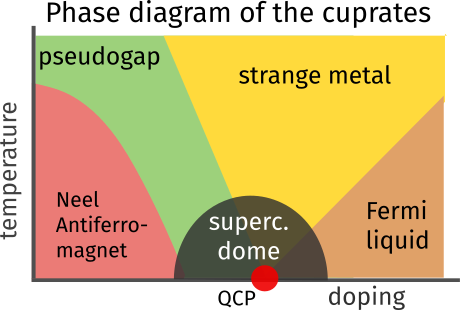
\includegraphics[width=\textwidth]{cuprates.pdf}
\end{minipage}

\vspace*{\fill}
% 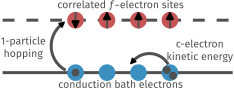
\includegraphics[width=0.5\textwidth]{periodicAnderson.pdf}
}
\only<2>{
\alert{Fractional Chern insulators}\\[5pt]
\begin{itemize}
	\item microscopic understanding of the FQHE ground states\\[10pt]
	\item emergence of composite degrees of freedom and topological theories
\end{itemize}

\vspace*{\fill}
% 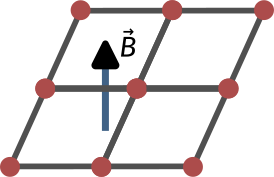
\includegraphics[width=0.3\textwidth]{ChernInsulator.pdf}
}
\only<3>{
\alert{Classification of RG flows in fermionic models}\\[5pt]
\begin{itemize}
	\item growth of multipartite entanglement towards stable fixed points\\[10pt]
	\item extending this to impurity models\\[10pt]
	\item connections with the URG noise operator
\end{itemize}
}
\end{frame}

\begin{frame}[c]{}
	\LARGE{THANK YOU.}
\end{frame}

\end{document}
